\newpage
\section{Rummets karakteristik}
En af CLIO-Pockets andre funktioner er, at den er i stand til, at måle impulsresponset i et rum. Dette blev gjort ved, at indstille softwarens parametre som der stod beskrevet i manualen og herefter lavet et 'klap' foran CLIO-mikrofonen. Resultatet af dette kan ses på figuren nedenfor:
\begin{figure}[H]
	\centering
	\vspace{-12pt}
	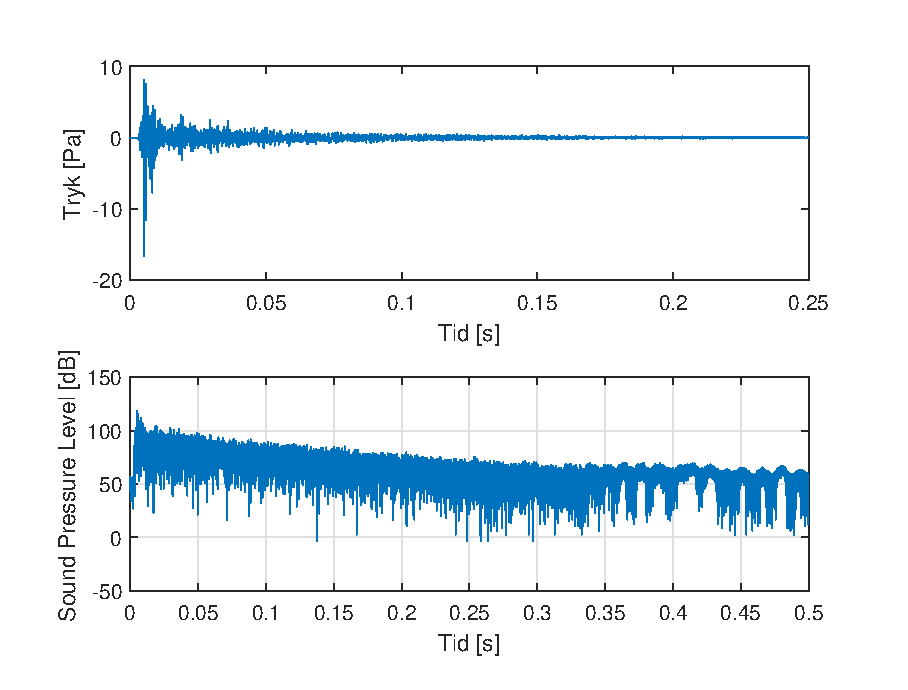
\includegraphics[width=\textwidth]{Billeder/Grafer/ImpulsResponse}
	\caption{Rummets impulsrespons i tids- og frekvensdomænet}
\end{figure}

\newpage
Tekst
\begin{figure}[H]
	\centering
	\vspace{-12pt}
	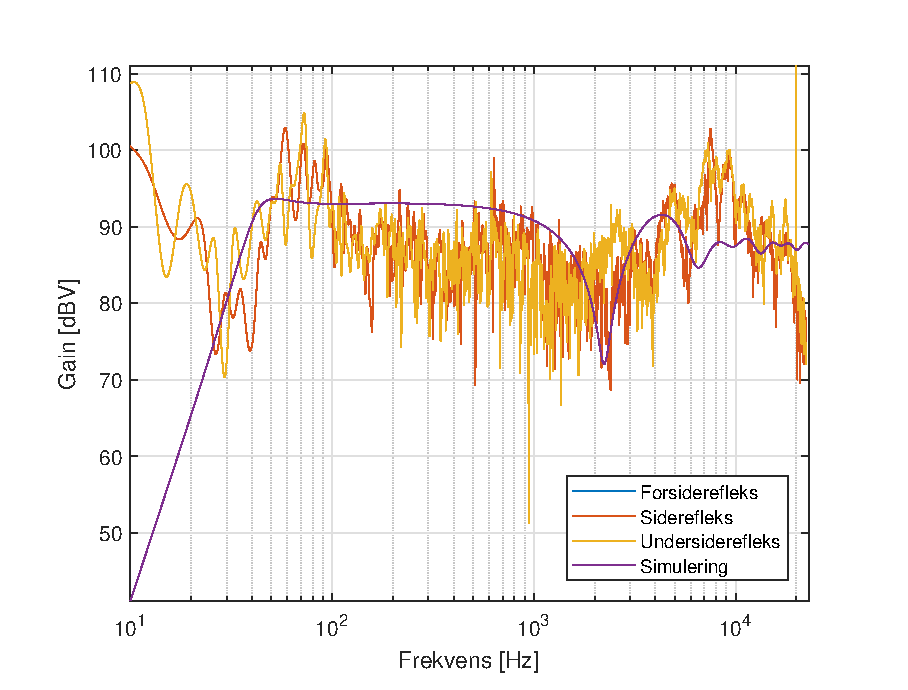
\includegraphics[width=\textwidth]{Billeder/Grafer/RealDirect}
	\caption{Rummets impulsrespons i tids- og frekvensdomænet}
\end{figure}

\newpage
Tekst
\begin{figure}[H]
	\centering
	\vspace{-12pt}
	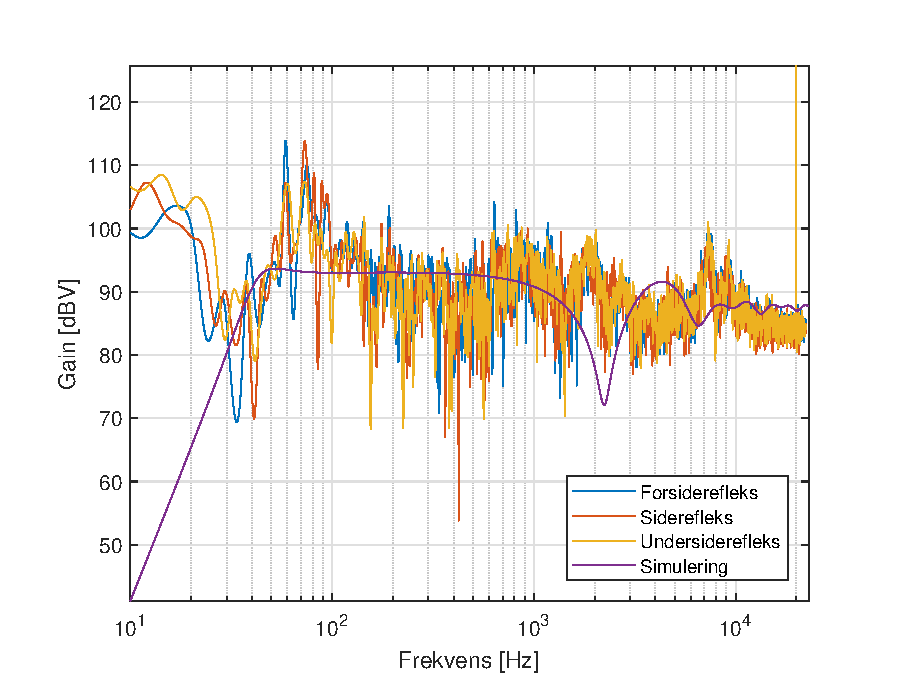
\includegraphics[width=\textwidth]{Billeder/Grafer/RealListen}
	\caption{Rummets impulsrespons i tids- og frekvensdomænet}
\end{figure}